% CC-BY-4.0; Copyright (c) 2026 Jonathan Yantis. Generated by tools/verify_power.py
\documentclass[border=5pt]{standalone}
\usepackage{pgfplots}
\pgfplotsset{compat=1.18}
\definecolor{studyblue}{RGB}{39,83,109}
\definecolor{studyorange}{RGB}{180,94,32}
\begin{document}
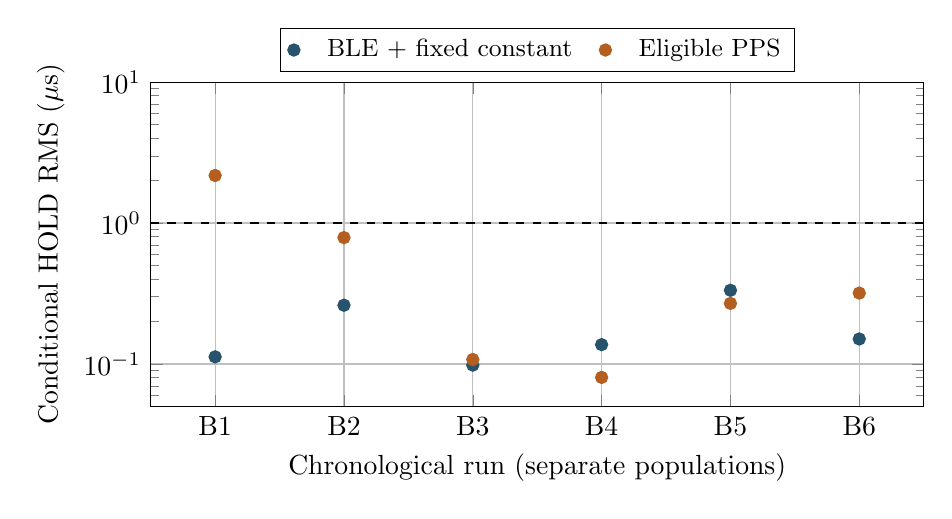
\begin{tikzpicture}\begin{semilogyaxis}[width=.94\linewidth,height=5.7cm,ymin=.05,ymax=10,xmin=.5,xmax=6.5,xtick={1,2,3,4,5,6},xticklabels={B1,B2,B3,B4,B5,B6},ylabel={Conditional HOLD RMS ($\mu$s)},xlabel={Chronological run (separate populations)},legend style={column sep=.8em,font=\small,at={(.5,1.03)},anchor=south,legend columns=2},grid=major]
\addplot[studyblue,thick,only marks,mark=*] coordinates {(1,0.1123315811) (2,0.2609765626) (3,0.09809248071) (4,0.1371132009) (5,0.3332209654) (6,0.1503965518)};\addlegendentry{BLE + fixed constant}
\addplot[studyorange,thick,only marks,mark=*] coordinates {(1,2.173739217) (2,0.7881964524) (3,0.1075357615) (4,0.08025926738) (5,0.2689882618) (6,0.3181796152)};\addlegendentry{Eligible PPS}
\addplot[black,dashed,forget plot] coordinates {(.5,1)(6.5,1)};
\end{semilogyaxis}\end{tikzpicture}
\end{document}
